\section{Précision de la verrerie (4 points)}

Voici deux instruments de mesure :

\begin{center}
	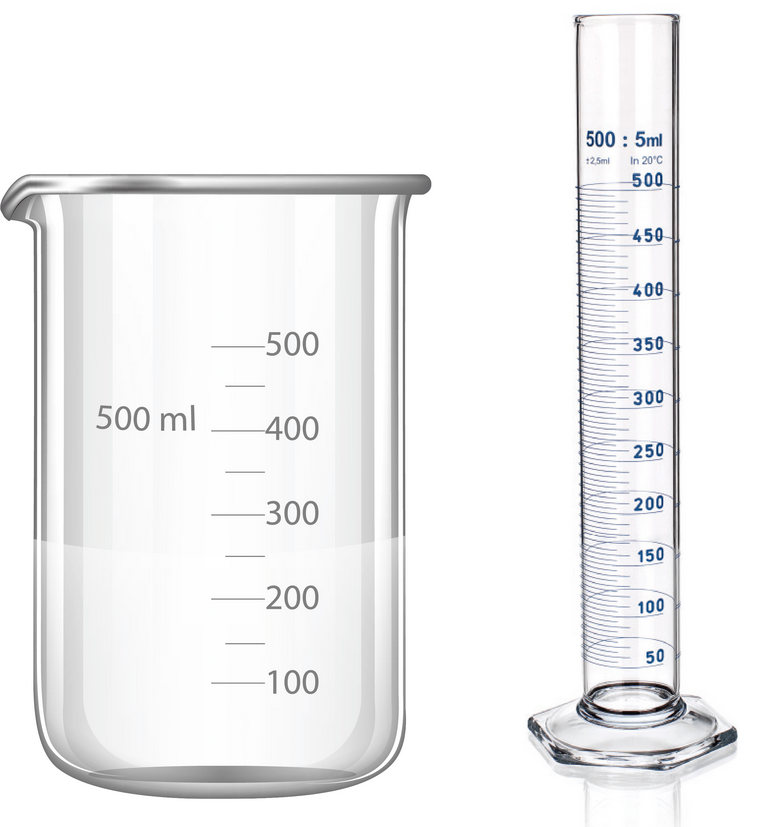
\includegraphics[scale=0.4]{img/vol}
\end{center}

\begin{questions}
	\question[1] Quel est leur nom ?

		\begin{solution}
			Le premier instrument est une bécher et le second une éprouvette graduée.
		\end{solution}
	
	\question[1] Quelle est l'unité de mesure utilisée pour ces instruments de mesure ?
	
	\begin{solution}
		Ils sont gradués en millilitres.
	\end{solution}

	\question[1] Dans chaque cas, à quel volume correspond un intervalle ?
	\begin{solution}
		Pour le bécher, il y a deux intervalles entre 400 et 500 mL. 
		
		\begin{equation*}
			\frac{500 - 400}{2} = 50
		\end{equation*}
		Donc un intervalle correspond à 50 mL.
		
		Pour l'éprouvette graduée, comme indiqué dessus, un intervalle correspond à 5 mL.
	\end{solution}
	
	%\question[1] Si l'on se trompe d'une graduation, quelle sera l'erreur commise sur la mesure ?
	
	\question[1] Lequel de ces instruments permet d'effectuer la mesure la plus précise ?
	\begin{solution}
		L'instrument qui permet d'effectuer la mesure la plus précise est celui pour lequel un intervalle correspond au plus petit volume. C'est donc l'éprouvette graduée.
	\end{solution}
	
%	\question Existe-t-il une relation entre le diamètre de l'instrument de mesure et la précision des mesures ?

\end{questions}